\documentclass[10pt]{report}
\usepackage[a4paper, height=10in, width=8in, hmargin={2cm,0.8in}]{geometry}
\usepackage{graphicx} % Required for inserting images
\usepackage{xeCJK}
\usepackage{amssymb}
\usepackage{amsthm}
\usepackage{amsmath}
\usepackage{caption}
\usepackage{comment}
\usepackage{subcaption}
\usepackage{enumerate}
\usepackage{multirow}
\usepackage{physics}
\usepackage[separate-uncertainty=true]{siunitx}
\usepackage{multirow}
\usepackage{booktabs}
\usepackage{chemformula}
\usepackage{sectsty}
\usepackage{svg}
\usepackage{url}
\usepackage{titlesec}
\usepackage{fontenc}

\newcommand{\chapfnt}{\fontsize{16}{19}}
\titleformat{\chapter}[hang]
{\normalfont\chapfnt\bfseries}{\thechapter}{20pt}{\chapfnt}

\setCJKmainfont{NotoSansTC-Regular}
\renewcommand{\baselinestretch}{1.25}

\title{112-2 近代物理實驗\\He-Ne Laser Comprehensive\\\vspace{1cm}
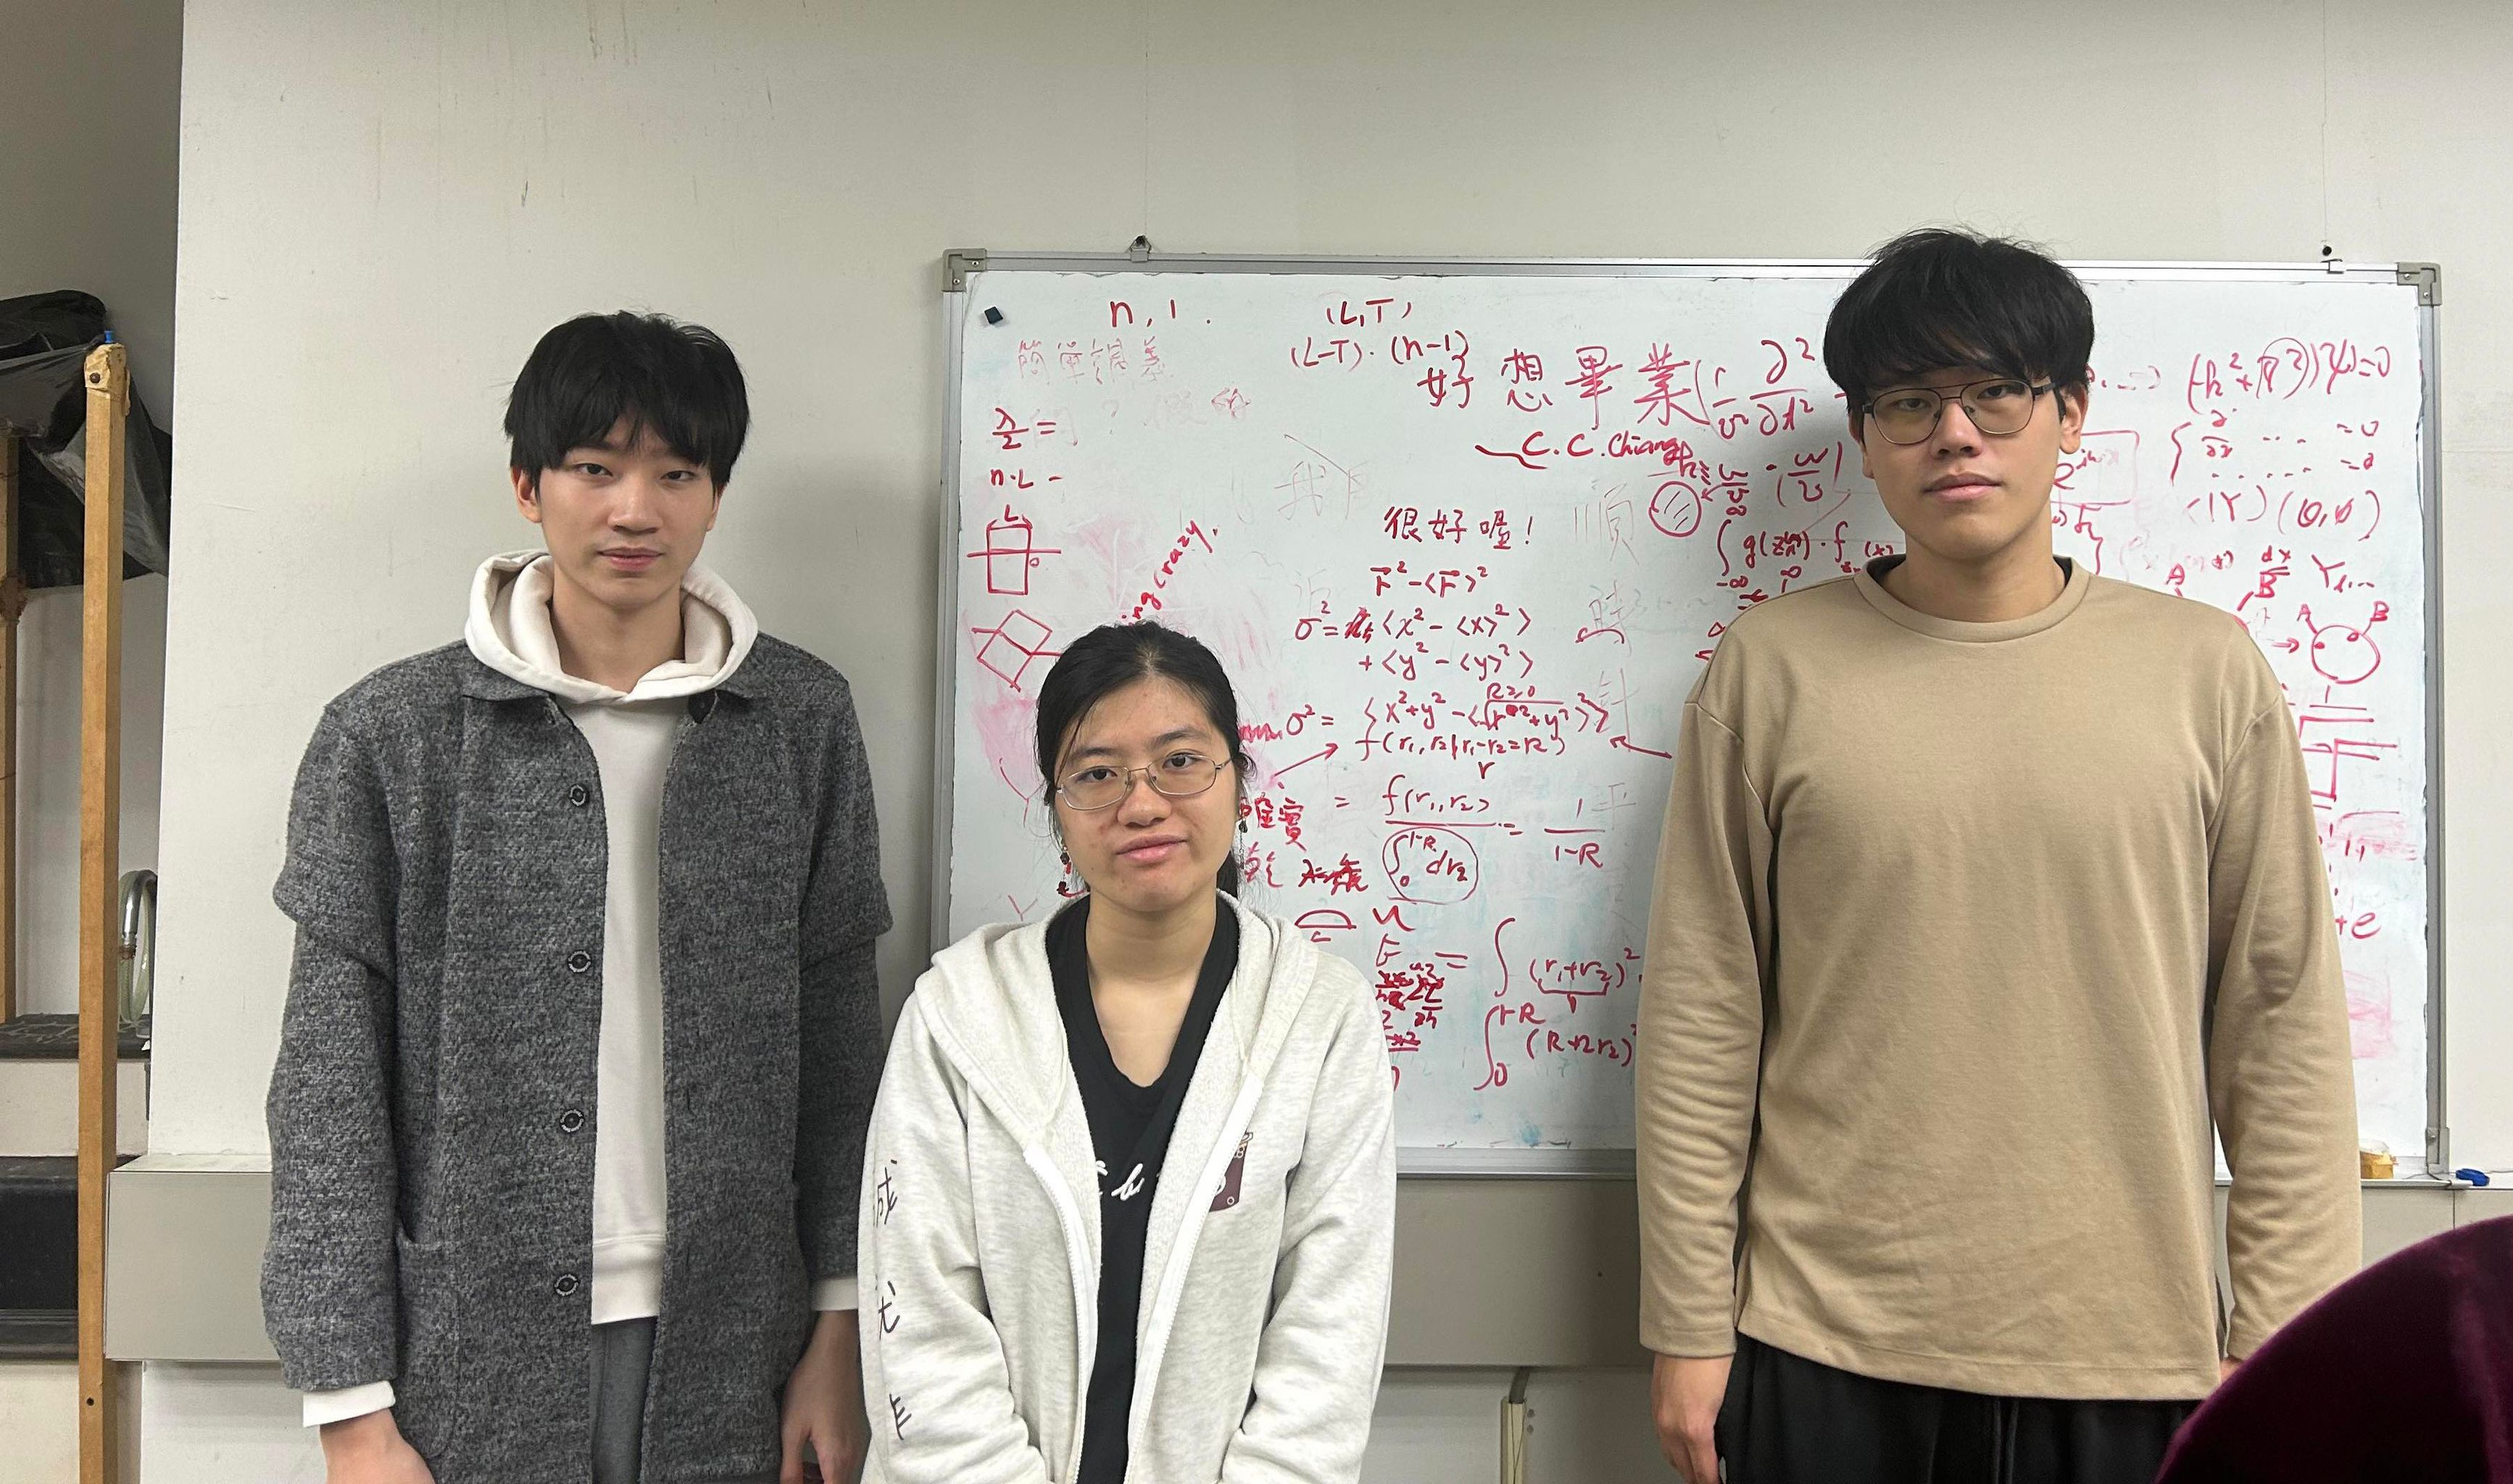
\includegraphics[width=0.5\textwidth]{Group photo}
}
\author{週一班第二組 \\ 左:林馳耘 B10202037 中:吉芸萱 B10202036 右:丁安磊 B10202051}
\date{實驗日期:05/13 \& 05/20 \& 05/27\\提交日期: 06/10}

\begin{document}

\renewcommand{\figurename}{圖}
\renewcommand{\tablename}{表}
\newcommand{\br}[1]{\left(#1\right)}
\renewcommand{\vb}[1]{\boldsymbol{\mathbf{#1}}} % New vector bold command to adapt for greek letters.

\maketitle

\tableofcontents

\clearpage

\chapter{氦氖雷射共振腔調整實驗}

\section{實驗原理}

\section{實驗步驟與觀察紀錄}

通過尺規板中心小孔,目視氦氖雷射毛細腔。調整尺規板小孔的位置,
使得自己可以看到毛細管中發光的 He-Ne 氣體所產生的大亮斑,調整尺規
板位置盡量使大亮斑成同心圓,這時看著亮斑左右移動尺規板座,你會發
現當時眼睛適應光線後,大亮斑中還有一個不太明顯的小亮斑在立體的移
動,這是毛細管另一端的反射鏡所反射回來的小光點,移動調整尺規板座,
我們將小亮斑調整到大亮斑的正中心,這時候理想上,我們的小孔是在毛
細管指的路徑上。

"一開始我們花很久時間在調半外腔的部分,後來我們發現是我們認知的最
小白色光斑跟講義認知的不同,在修正認知之後每次就能快速調出光。"

\section{結果與討論}

\chapter{共焦球面掃描干涉儀調整實驗}

\chapter{氦氖半外腔等效腔長測量實驗}

\chapter{雷射橫模變換與參數測量實驗}

\chapter{氦氖雷射縱模正交偏振與模式競爭觀測實驗}

\chapter{高斯光束基本參數測量實驗}

\chapter{高斯光束的傳播特性實驗}

\chapter{高斯光束擴束及準直實驗}

\chapter{光束品質分析實驗}

\chapter{雷射共振腔設計實驗}

\bibliographystyle{unsrt} % We choose the "plain" reference style
\bibliography{ref.bib} % Entries are in the refs.bib file

\end{document}